Consider a more practical approach that takes all the previously discussed aspects.
Applying modern frameworks like ASP .NET Core, Angular etc.
let be the following authentication flow as per diagram below
\begin{figure}[H]
    \centering
    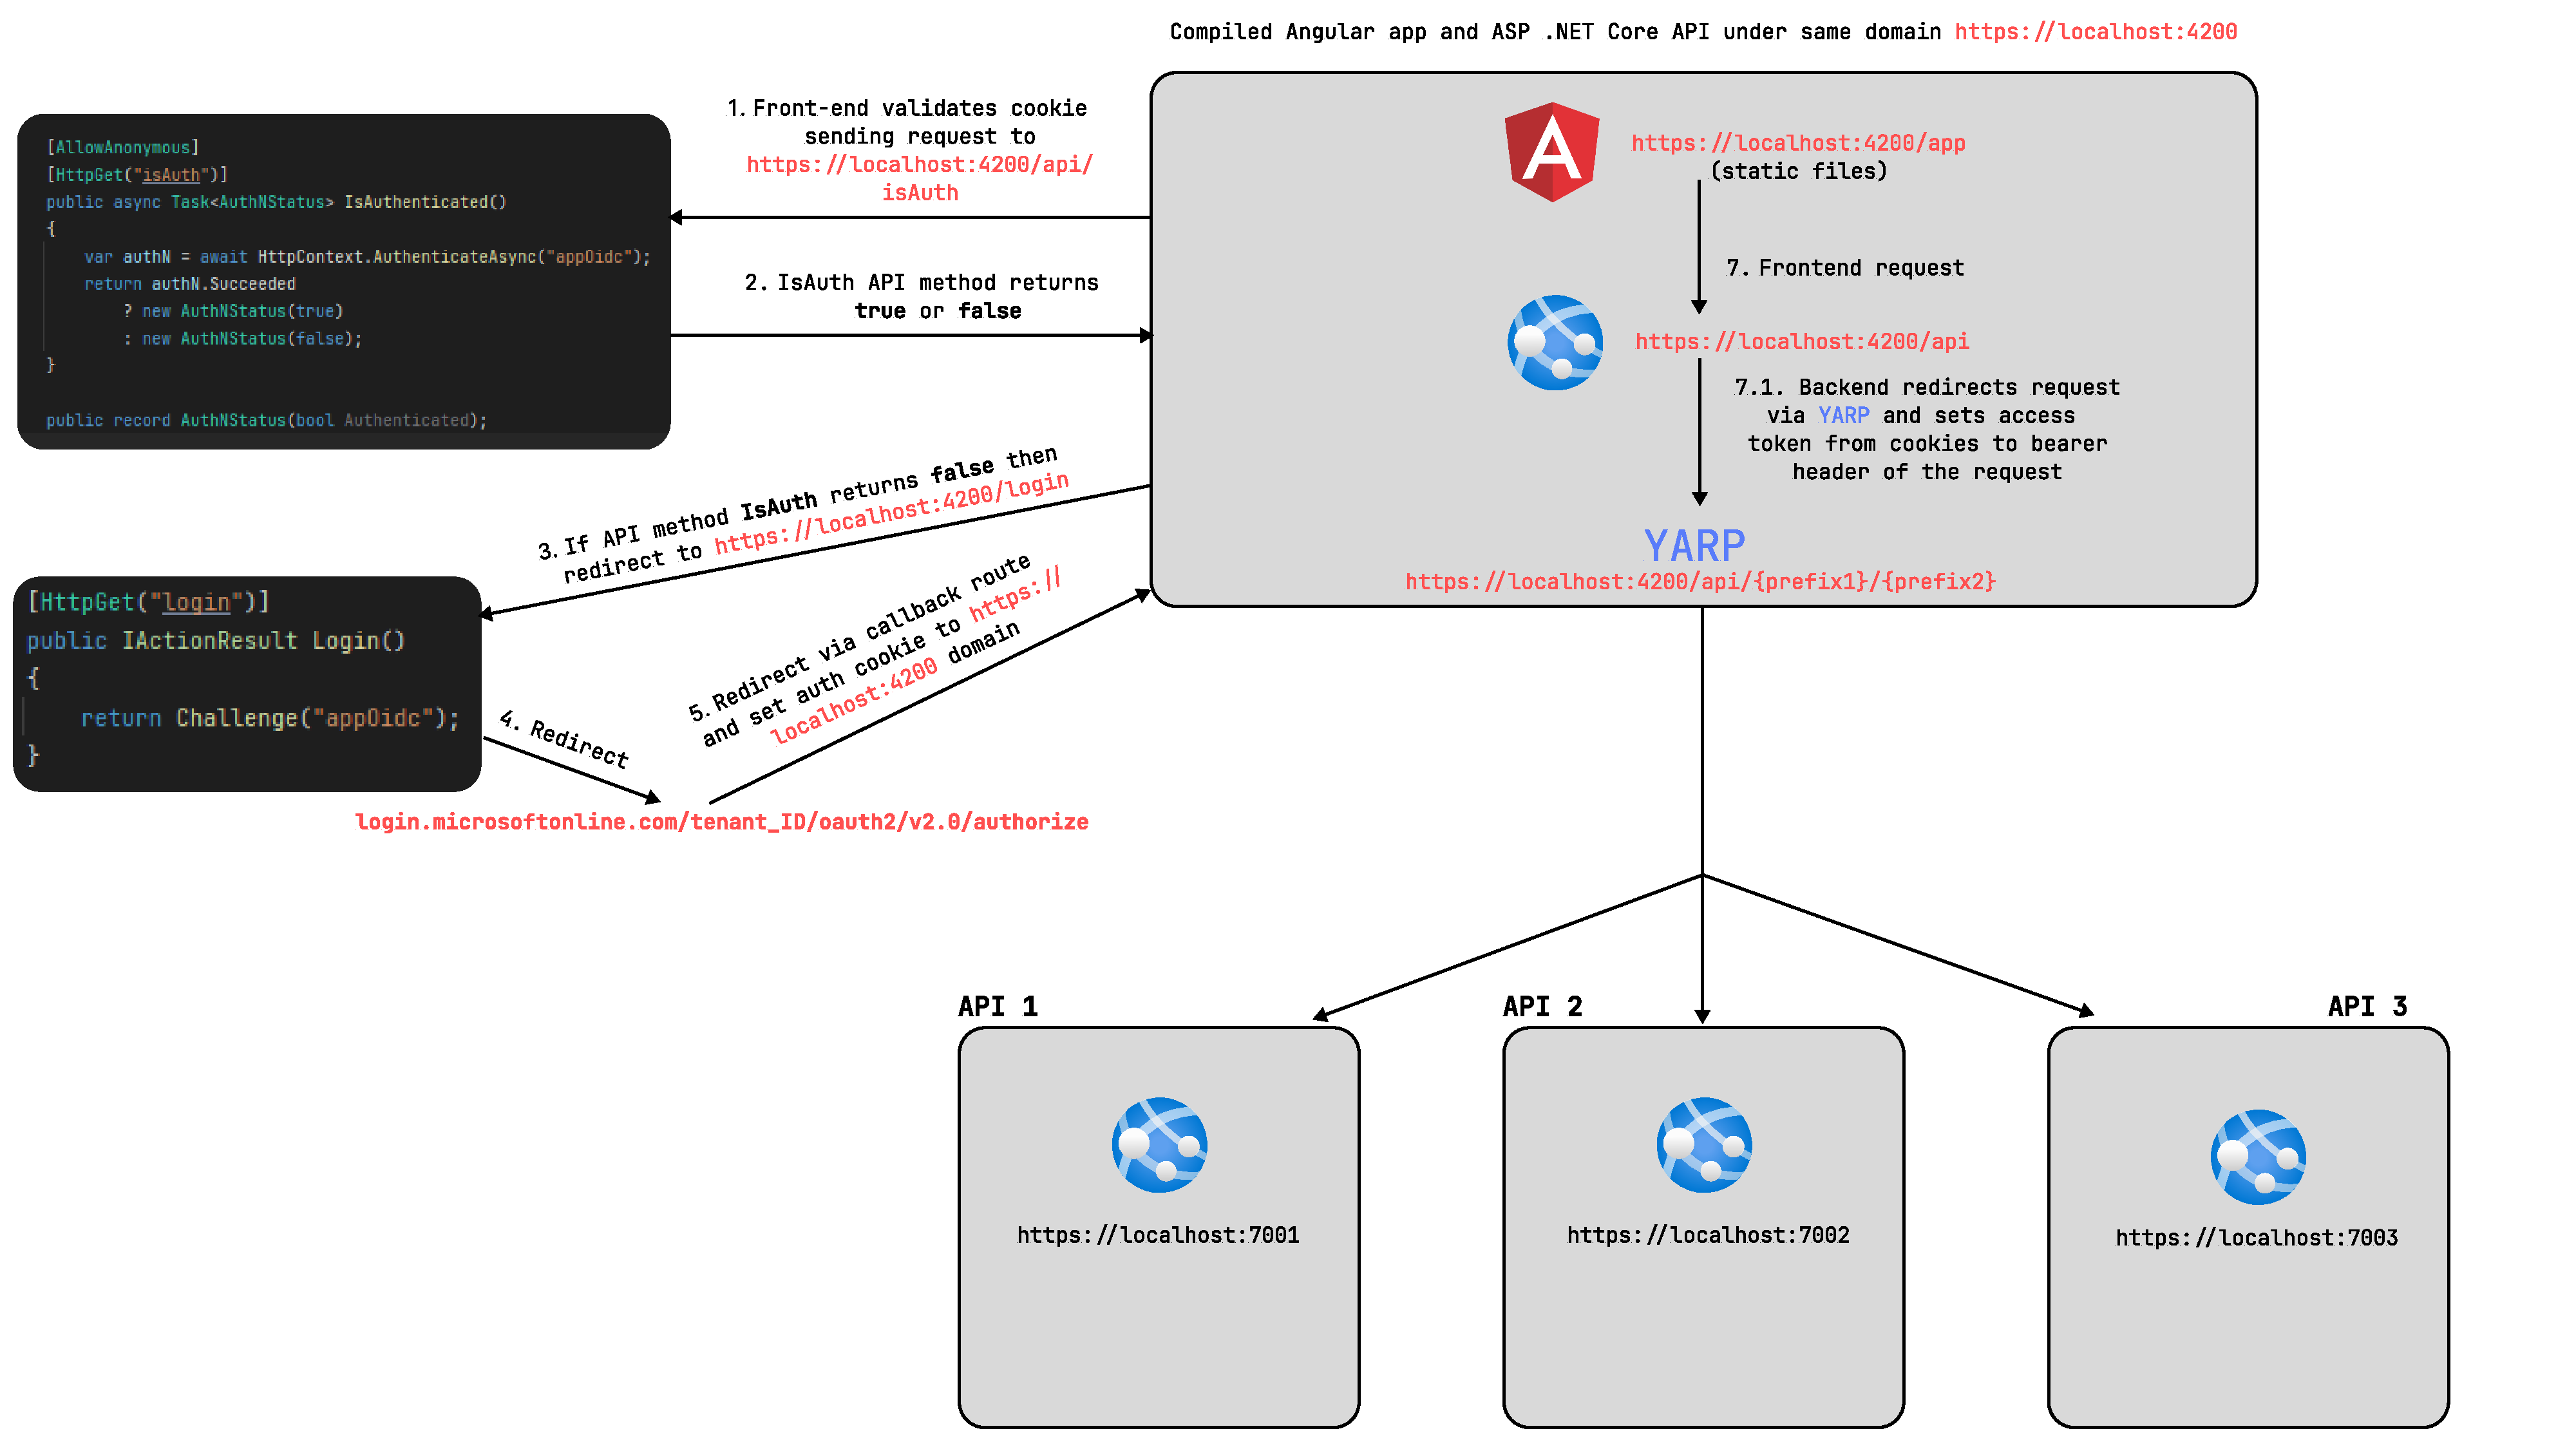
\includegraphics[width=1\textwidth]{img/Auth_flow_updated}
    ~\caption{Authentication flow diagram.}\label{fig:authentication_flow_diagram}
\end{figure}

Therefore, the whole authentication process can be described as nine steps such that
\begin{enumerate}
    \item Compiled Angular frontend application sends request to the authentication endpoint of the ASP .NET Core API
    to verify current authentication state.
    Angular application is a set or precompiled bundles that are exposed via same ASP .NET Core API
    so that cross-origin requests are not necessary and tokens can be stored in cookie files securely.
    \item Authentication endpoint of the ASP .NET Core API responses either with
    HTTP status code \texttt{200 (OK)} or \texttt{401 (Unauthorized)}
    \item If \texttt{401 (Unauthorized)} status code received from previous step,
    then browser is redirected to the \texttt{login} endpoint of the ASP .NET Core API,
    otherwise user gets access to the protected resources
    \item Login method of the ASP .NET Core API redirects browser to the Azure AD authorize url
    \texttt{login.microsoftonline.com/tenant/oauth2/v2.0/authorize} where user enters his credentials
    \item If user is logged in then browser is redirected to fallback url with cookies already set for \texttt{https://localhost:4200} domain
    \item Request is sent to validate authentication \texttt{https://localhost:4200/api/isAuth}, now it returns \texttt{true}
    \item Frontend at \texttt{https://localhost:4200/app} sends request to the \\ \texttt{https://localhost:4200/api/OtherApi1/products}
    \item Cookie exists for \texttt{https://localhost:4200/app} so that \\ \texttt{https://localhost:4200/api}
    attaches it as header to request via YARP and sends request with token to the external resource \texttt{OtherApi1/products}
    \item If response code is 401 at step (8) then repeat step (1)
\end{enumerate}